\mychapter{state-of-the-art}{State of the Art in Provisioning}

There already exists scientific research projects, APIs, frameworks 
and other technologies which aim at consolidating, interfacing and utilizing cloud technologies.
This chapter introduces some of these concepts.
First scientific research projects will be presented with their solutions, 
then pure technological approaches will be introduced.

\section{Model-Driven Approaches}

The following technologies are in some way model based.
That means they either use concrete diagrams or any other means of
modeling that can relate to Model-Driven Engineering.

\paragraph{Amazon AWS CloudFormation.}~\cite{aws}

\begin{figure}[tb]
  \begin{center}
    \begin{minted}[mathescape,
                   linenos,
                   numbersep=5pt,
                   frame=lines,
                   framesep=2mm]{json}
{
  "Description": "Create an EC2 instance",
  "Parameters": {
    "KeyPair": {
      "Description": "For SSH access",
      "Type": "String"
    }
  },
  "Resources": {
    "Ec2Instance": {
      "Type": "AWS::EC2::Instance",
      "Properties": {
        "KeyName": { "Ref": "KeyPair" },
        "ImageId": "ami-1234abcd" 
      }
    }
  },
  "Outputs" : {
    "InstanceId": {
     "Description": "Instace ID of created instance",
     "Value": { "Ref": "Ec2Instance" }
    }
  },
  "AWSTemplateFormatVersion": "2010-09-09"
}
    \end{minted}
  \end{center}
  \caption{AWS CloudFormation template.}
  \label{fig:cloudformation-template}
\end{figure}



This is a service provided by Amazon from their popular \myac{AWS}.
It give users the ability to create template files in form of 
\myac{JSON} as seen in ~\citefig{cloudformation-template}, 
which they can load into AWS to create stacks of resources. 
A \emph{stack} is a defined set of resources in different amount and sizes, 
such as numerous instances,
one or more databases and a load balancer, although what types and sizes of resources is ambiguous.
To provision a stack with CloudFormation the template file (in JSON format) is first uploaded to
AWS which makes it accessible from AWS Management Console.

The template consist of three main sections, 
\begin{ii}\iitem \emph{Parameters}, \iitem \emph{Resources} and \iitem \emph{Outputs}.\end{ii}
The \emph{Parameters} section makes it possible to send parameters into the template, 
with this the template becomes a macro language by replacing 
references in the \emph{Resources} section with inputs from users. 
Input to the parameters are given inside the management console when 
provisioning a stack with a given template.
The \emph{Resource} section define types of resources that should be provisioned, the \emph{Type}
property is based on a set of predefined resource types such as \emph{AWS::EC2::Instance}
in Java package style.
The last section, \emph{Output}, will generate output to users when provisioning is complete,
here it is possible for users to pick from a set of variables to get the information they need.

This template system makes it easier for users to duplicate a setup many times, 
and as the templates support parameters this process can be as dynamic as the user design it to be. 
This is a model in form or lexical syntax, both the template itself 
and the resources that can be used.
For a company that is fresh in the world of cloud computing this service 
could be considered too advance. 
This is mainly meant for users that want to replicate a certain stack, 
with the ability to provide custom parameters. 
Once a stack is deployed it is only maintainable through the AWS Management Console, 
and not through template files. 
The format that Amazon uses for the templates is a good format, 
the syntax is in form of JSON which is readable and easy to use, 
but the structure and semantics of the template itself is not used by any 
other providers or cloud management tooling, 
so it can not be considered a multicloud solution. 
Even though JSON is a readable format, 
does not make it viable as a presentation medium on a business level.

\paragraph{CA Applogic.}~\cite{applogic}

\begin{figure}
  \begin{center}
  \end{center}
  \caption{CA Applogic}
    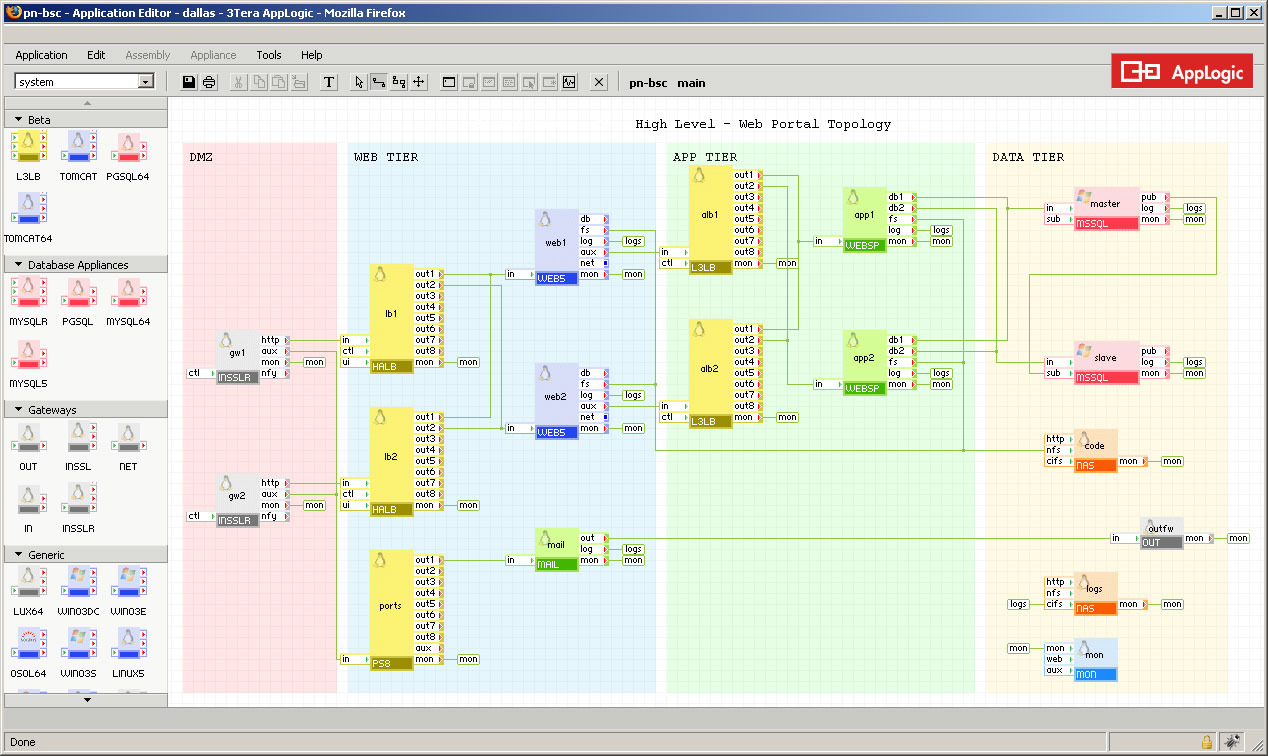
\includegraphics[width=\linewidth]{img/applogic.jpg}
  \label{fig:applogic}
\end{figure}


The Applogic platform is designed to manage CAs private cloud 
infrastructure~\cite{introducing-cloud-services}.
It also has a web based interface which let users manage their cloud resources 
as shown in~\citefig{applogic} which use and benefit from a model based approach.
It is based on graphical models which support interactive ``drag and drop'' functionalities.
This interface let users configure their deployments through a diagram with familiarities to 
UML component diagrams with interfaces and assembly connectors. 
They let users configure a selection of third party applications, 
such as Apache and MySQL, as well as network security, instances and monitoring. 
What CA has created is both an easy way into the cloud and it utilizes 
the advantages of model realizations. 
Their solution will also prove beneficial when conducting business level consulting
as it visualizes the structural layout of an application.
But this solution is only made for private clouds running their own controller, 
this can prove troublesome for migration, both in to and out of the infrastructure.

\section{APIs}

Extensive work have been done towards simplifying and combining cloud technologies through
abstractions, interfaces and integrations.
Much of this work is in form of APIs, mostly in two different forms.
Either as programming libraries that can be utilized directly from a given 
programming language or environment such as Java or Python.
The other common solution is to have an online facade against public providers,
in this solution the APIs are mostly in RESTful form.
APIs can be considered modeling approaches based on the fact they have a topology 
and hierarchical structure, 
but it is not a distinct modeling. 
A modeling language could overlay the code and help providing a clear overview, 
but the language directly would not provide a good overview of deployment. 
And links between resources can be hard to see, 
as the API lacks correlation between resources and method calls. 

\subparagraph{Driver.}

\begin{figure}[tb]

  \begin{tikzpicture}[scale=1, transform shape]
    \node (Framework) [box, minimum width=8cm, minimum height=5cm] { };

    \node (Interface) [class, text width=2cm, yshift=0.25cm, xshift=-2.5cm] { 
      \textbf{Common  \\ interface} 
    };

    \node (Driver-EC2) [class, right=of Interface] { 
      \textbf{Driver - EC2} 
    };
    \node (Driver-Rackspace) [class, above=of Driver-EC2] { 
      \textbf{Driver - Rackspace} 
    };
    \node (Driver-Azure) [class, below=of Driver-EC2] { 
      \textbf{Driver - Azure} 
    };

    \node (EC2) [tcloud, xshift=1cm, right=of Driver-EC2] { \textbf{EC2} };
    \node (Rackspace) [tcloud, xshift=1cm, right=of Driver-Rackspace] { \textbf{Rackspace} };
    \node (Azure) [tcloud, xshift=1cm, right=of Driver-Azure] { \textbf{Azure} };

    \draw[arrow] (Interface) -- (Driver-EC2.west);
    \draw[arrow] (Interface) -- (Driver-Rackspace.west);
    \draw[arrow] (Interface) -- (Driver-Azure.west);

    \draw[arrow] (Driver-EC2) -- (EC2);
    \draw[arrow] (Driver-Rackspace) -- (Rackspace);
    \draw[arrow] (Driver-Azure) -- (Azure);
  \end{tikzpicture}

  \caption{Cloud drivers.}
  \label{fig:drivers}
\end{figure}


Many of the API solutions use the term ``\emph{driver}'', it represents
a module or component that fit into existing software and extend the support
of external connections without changing the interface.
A cloud \emph{driver} connects a given software to an existing cloud provider
through this providers web based API (REST), illustrated in \citefig{drivers}.

\paragraph{jclouds.}~\cite{jclouds}

This is a library written in Java and can be used from any \myac{JVM}-based language.
Provider support is implemented in \emph{drivers}, and they even support deployments
to some \myac{PaaS} solutions such as \myac{GAE}.
\emph{jclouds} divide their library in two different parts, one for computing powers 
such as \myac{EC2} and one for blob storage like S3. 
Some blob storage services are accessible on the compute side of the library such
as \myac{EBS}.
They support ``dry runs'' so a stack can be deployed as a simulation, not 
actually deploying it to a public cloud.
This is beneficial for testing deployments, and writing unit tests without initializing
connections, the library enhance this by providing a stub aimed at testing.


\paragraph{libcloud.}~\cite{libcloud}

Libcloud is an API that aims to support the largest cloud providers through a common API. 
The classes are based around \emph{drivers} that extends from a common ontology, 
then provider-specific attributes and logic is added to the implementation.
Libcoud is very similar to jclouds but the API code base is written in Python. 
The API is Python-only and could therefor be considered to have high tool-chain dependency.

\paragraph{Deltacloud.}~\cite{deltacloud}

Deltacloud has a similar procedure as jclouds and libcloud, but with a REST API. 
So they also work on the term \emph{driver}, but instead of having a library to a 
programming language the users are presented with an web-based API they can call
on Deltacloud servers. 
As well as having similar problems as other APIs this approach means 
that every call has to go through their servers, similar to a proxy. 
This can work with the benefits that many middleware softwares have, such as caching, queues, 
redundancy and transformations.
The main disadvantages are single point of failure and version inconsistencies.
Deltacloud provide two sets of native libraries, one in Ruby and another in C, which
makes it easier to communicate with the REST API.
Previously discussed \emph{jclouds} also support Deltacloud, as it would interface this
with a \emph{driver} as any other web-based API.


\section{Deployments}

There are also some solutions that specifically aim at full deployments,
contra provisioning single instances or services these solutions
provision everything needed to fully deploy an application with a given ontology.

\paragraph{mOSAIC.}~\cite{portable:petcu12} 

Aims at not only provisioning in the cloud, but deployment as well.
They focus on abstractions for application developers and state they can easily enable users to
\emph{``obtain the desired application characteristics (like
scalability, fault-tolerance, QoS, \etc.)''}~\cite{architecturing:petcu11}.
There are two abstraction layers, one for cloud provisioning 
and one for application-logic.
mOSAIC will select a proper cloud based on how developers describe their application.
Several clouds can be selected based on their properties, then communication between
these clouds will be done using ``cloud based message queues technologies''.

\paragraph{reservoir.}~\cite{reservoir:rochweger09}

Another project that also aim at multicloud. 
The other goals of this project is to leverage 
scalability in single providers and support built-in \myac{BSM}.

\paragraph{Vega.}~\cite{simplifying:chieu10} 

Vega framework is a deployment framework aiming 
at full cloud deployments of multi-tier topologies, 
they also follow a model-based approach. 
The description of a given topology is done by using XML files, with these files
developers can replicate a \emph{stack}.
A resource manager keep track of resources in a system, grouping instances after their attributes.

\section{\todo{Languages and technologies}}

\note{Bad section name?}

\paragraph{EC2}

\todo{Should I write about EC2?}

\paragraph{OPA.}~\cite{opa}

OPA is a cloud language aimed at easing development of modern web applications. 
The language will build into executable files that will handle load balancing and scalability, 
this is to to make this a part of the language and compilation.
It will also handle communication between client and server, the client side part of OPA
is generated into JavaScript.
OPA is a new language, so it might be difficult to migrate legacy systems into this language. 
There are no deployment configurations, as this is built into the language. 
The conclusion about OPA is that it is not a language meant for configuration, 
and could not easily benefit from a model based approach, 
and it does not intentionally solve multicloud.
The benefit is that make building new web based applications is easier and more concrete.
Another strong side is that OPA handle security vulnerabilities by default,
such as SQL injections or XSS attacks.

\paragraph{Amazon Beanstalk.}

Amazon has been known for providing IaaS solutions (EC2) and services complementing 
either their IaaS or the \emph{Storage as a Service} solution S3.
Unlike some providers such as Microsoft and Google they had yet to introduce
a PaaS based solution, until they created Beanstalk.
This is the Amazon answer to PaaS, it is based on pre-configuring 
a stack of existing services such as \myac{EC2} for computing, 
\myac{EBS} for storage and \myac{ELB} for load balancing.
At the writing moment they support Java with Tomcat and PHP deployments.
The Java solution is based on uploading war-files to Beanstalk, then 
the service will handle the rest of the deployment.
For PHP the deployment is based on GIT repositories, when pushing
code to a given repository Beanstalk will automatically deploy the new code
to an Apache httpd instance.

